\documentclass[11pt, a4paper, titlepage, twoside]{article}

\usepackage[utf8]{inputenc}
\usepackage[T1]{fontenc}
\usepackage[USenglish]{babel}

\renewcommand{\emph}{\textbf}
\usepackage{cmbright}

\usepackage[a4paper, left=3cm, right=3cm, top=3.5cm, bottom=3.5cm]{geometry}
\usepackage[automark, headsepline, footsepline]{scrpage2}
\usepackage{indentfirst}
\usepackage{graphicx}
\usepackage[labelfont=bf, textfont=it]{caption}
\usepackage{setspace}
\usepackage[nottoc]{tocbibind}

\newcommand{\version}{1.2.1}

\usepackage[
	pdftitle = {SortSimulation},
	pdfsubject = {Documentation},
	pdfauthor = {Peter\ {}Folta},
	pdfkeywords = {},
	pdfcreator = {},
	pdfproducer = {},
	colorlinks = true,
	linkcolor = black,
	anchorcolor = black,
	citecolor = black,
	filecolor = black,
	menucolor = black,
	pagecolor = black,
	urlcolor = blue]{hyperref}

\usepackage{listings}
\renewcommand{\lstlistingname}{Listing}
\renewcommand{\lstlistlistingname}{Listings}
\lstset{basicstyle=\ttfamily, tabsize=4, numbers=left, numberstyle=\scriptsize, xleftmargin=20pt}

\title{SortSimulation}
\author{Peter Folta}

\clearscrheadfoot
\ihead[\headmark]{\headmark}
\ohead[\pagemark]{\pagemark}
\ifoot[SortSimulation~-- Documentation]{SortSimulation~-- Documentation}
\ofoot[Version \version]{Version \version}

\pagestyle{scrheadings}

\onehalfspacing

\begin{document}
	\pagenumbering{roman}
	
	\begin{titlepage}
		\begin{center}
			\vspace*{2.5cm}
			\Huge{\textbf{SortSimulation}}
			
			\vspace*{1.5cm}
			\LARGE{Documentation}
			
			\Large{-- English --}
			
			\vspace*{3.75cm}
			\Large{Peter Folta}
		\end{center}
		
		\vspace*{8cm}
		\noindent{}Version \version\newline{}
		Internet: \href{http://www.peterfolta.de/software/sortsimulation}{http://www.peterfolta.de/software/sortsimulation}\newline{}
		Copyright \textcopyright{} 2008--2009 Peter Folta. All rights reserved.
	\end{titlepage}
	
	\setcounter{page}{2}
	
	\cleardoublepage{}
	\tableofcontents{}
	\newpage{}
	
	\pagenumbering{arabic}
	
	\section{Introduction}
	
	SortSimulation is a java application, that visualizes different sorting algorithms. This gives you a better understanding of their operating mode and illustrates runtime differences without just comparing dull numbers.
	
	\begin{figure}[h]
		\begin{center}
			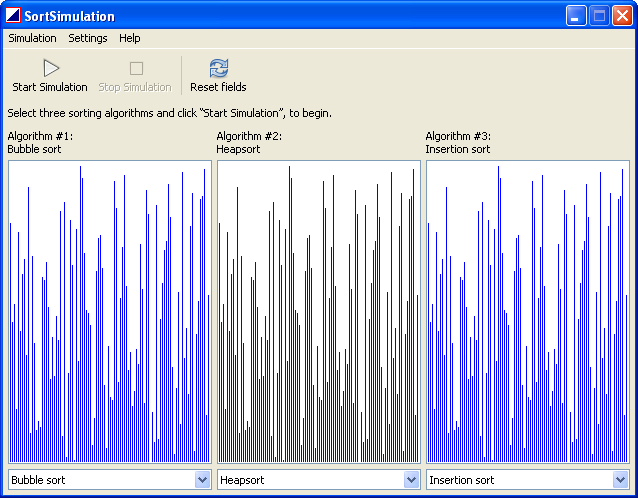
\includegraphics[scale=0.6]{images/image0.png}
			\caption{Main window of SortSimulation}
		\end{center}
	\end{figure}
	
	This documentation contains a brief introduction into the usage of SortSimulation and presents you with the supported sorting algorithms including their java implementation.
	
	\section{Usage}
	
	Using SortSimulation is really simple: The sorting fields are randomly filled right after the program launch---every field contains the same initial situation. Three sorting algorithms are also preselected just after the program launch.
	
	To compare three particular sorting algorithms, select them from the combo boxes below the fields. Click on \emph{Start simulation} in the toolbar or the menu, or press the enter key on your keyboard alternatively, to begin. Cancelling an active simulation is just as easy: Press the escape key or click on \emph{Stop simulation}. To reset the fields after a finished or cancelled simulation, click on the button \emph{Reset fields} or press \texttt{Ctrl+N}.
	
	SortSimulation allows you to configure the simulation as you wish. The available settings are discussed in the following paragraph.
	
	\subsection{Settings}
	
	SortSimulation offers you miscellaneous options to configure the sorting simulations in the way you want it. The available settings are listed in the menu \emph{Settings}:
	
	\begin{figure}[h]
		\begin{center}
			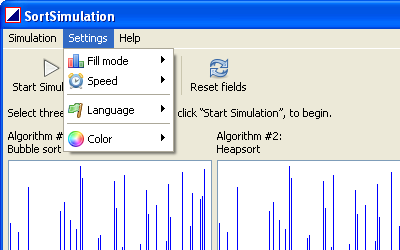
\includegraphics[scale=0.6]{images/image1.png}
			\caption{The settings menu}
		\end{center}
	\end{figure}
	
	To configure the way the sorting fields are filled, the option \emph{Fillmode} offers you two possibilities: Randomly (preselected; \texttt{Ctrl+R}) and Inverse (\texttt{Ctrl+I}). If \emph{Randomly} is selected, the elements are ordered randomly in the fields when the user commits the action \emph{Reset fields}. This allows you to try the different sorting algorithms on totally unsorted data in a realistic way.
	
	In contrast, the mode \emph{Inverse} fills the fields already sorted---but backwards (descending instead of ascending). Using this setting gives you the possibility to take a closer look on the efficiency of the algorithms sorting backwards pre-ordered series.
	
	The submenu \emph{Speed} allows you to configure the speed of the simulation. You can choose the speed between five levels. While algorihms like Bubble sort are quite slow, it is worth to select one of the higher speed levels; while running a sorting algorithm like Quicksort, it's better to choose a slower speed to be able to take a closer look at the functionality. It's also possible to set the different speed levels by keyboard using the sortcuts \texttt{Ctrl+Shift+(1-5)}.
	
	SortSimulation doesn't create or modify any of the files stored on your computer, that's why SortSimulation's user interface language is always set to English after the program launch, even if you changed it before. To switch between the offered languages, go to the submenu \emph{Language}.
	
	The last submenu \emph{Color} is used to configure the color of the bars. Blue is set by default, but you have the choice between eight different colors.
	
	\section{Sorting algorithms}
	
	\subsection{Bubble sort}
	
	Bubble sort is a really simple sorting algorithm, that sorts elements using a \emph{step-by-step comparison}. Because bubble sort is not very efficient, it is often used to demonstrate a weak sorting algorithm.
	
	\subsubsection{Idea of Bubble sort}
	
	Bubblesort works by comparing two list items and swapping them if they are in the wrong order. This procedure is repeated until all elements are in the correct position.
	
	\subsubsection{Java implementation}
	
	\lstinputlisting[caption={Implementation of Bubble sort}, label=lst:bubblesort, captionpos=b]{../Listings/Bubblesort.java}
	
	\subsection{Heapsort}
	
	Heapsort is a fast sorting algorithm which was developed by \emph{Robert W Floyd} and \emph{J.\,W.\,J. Williams} in 1964. Heapsort is an improvement of \emph{Selection sort}.
	
	\subsubsection{Idea of Heapsort}
	
	Heapsort uses the \emph{heap} as a specialized data structure for sorting. This data structure is based on an (almost) complete \emph{binary tree}. A binary tree is (almost) complete, if all levels except possibly the last are completed.
	
	If the sequence exists as a heap, the largest element can be taken out of the \emph{root} of the tree. To get to the next item, the heap has to be \emph{rearranged} before.
	
	\subsubsection{Java implementation}
	
	\lstinputlisting[caption={Implementation of Heapsort}, label=lst:heapsort, captionpos=b]{../Listings/Heapsort.java}
	
	\subsection{Insertion sort}
	
	Insertion sort is a quite simple sorting algorithm. It is not as efficient as other more complex algorithms, but \emph{easy to implement} and has a very short run time in case of a small amount of data or already presorted data.
	
	\subsubsection{Idea of Insertion sort}
	
	Insertion sort removes an element of the unsorted set and inserts it in the correct place of the output sequence. If the sequence is empty, the element will be inserted at the first position.
	
	Insertion sort is inefficient, because this sorting algorithm often needs to move elements over long distances.
	
	\subsubsection{Java implementation}
	
	\lstinputlisting[caption={Implementation of Insertion sort}, label=lst:insertionsort, captionpos=b]{../Listings/Insertionsort.java}
	
	\subsection{Merge sort}
	
	Merge sort is a recursive and stable sorting algorithm, which is based on the \emph{divide and conquer principle}, like \emph{Quicksort}. Merge sort was presented by John von Neumann in 1945.
	
	\subsubsection{Idea of Merge sort}
	
	Merge sort splits the sequence into several smaller sequences, which will be sorted each for itself. After that the sorted, small sequences are united in one completly sorted sequence.
	
	\subsubsection{Java implementation}
	
	\lstinputlisting[caption={Implementation of Merge sort}, label=lst:mergesort, captionpos=b]{../Listings/Mergesort.java}
	
	\subsection{Quicksort}
	
	Quicksort is one of the \emph{fastest sorting algorithms}, based on the \emph{divide and conquer principle}. The recursive Quicksort algorithm in its original version was developed by \emph{C. Antony R. Hoare} in 1960.
	
	\subsubsection{Idea of Quicksort}
	
	The sequence will initially be split into two part. The first section contains all elements less than or equal to all elements in the second section (\emph{divide}). Then the two pieces are independently recursively sorted using the same procedure (\emph{conquer}). The last step combines the smaller sequences to a sorted one (\emph{combine}).
	
	The division is realized using a \emph{pivot element}, which is selected from the array in the first step. All elements of the sequence, which are \emph{smaller} than the pivot element, will be put in the first section. All the elements, that are \emph{larger} than the pivot element, will be put in the second section. For elements which have the same value as the pivot element, it does not matter in what part they are put.
	
	\subsubsection{Java implementation}
	
	\lstinputlisting[caption={Implementation of Quicksort}, label=lst:quicksort, captionpos=b]{../Listings/Quicksort.java}
	
	\subsection{Selection sort}
	
	Selection sort is a naive sorting algorithm that works in place. It is compareable to insertion sort.
	
	\subsubsection{Idea of Selection sort}
	
	Selection sort divides the sequence in a \emph{sorted} and a \emph{unsorted} field. The sorted part is empty at the beginning. Selection sort examines the smallest element in the unsorted part and swaps it with the first element. The sequence is sorted until this position after the step is made. The procedure is repeated until the entire sequence is sorted.
	
	\subsubsection{Java implementation}
	
	\lstinputlisting[caption={Implementation of Selection sort}, label=lst:selectionsort, captionpos=b]{../Listings/Selectionsort.java}
	
	\subsection{Shell sort}
	
	The sorting algorithm Shell sort is based on \emph{Insertion sort}. It was invented in 1959 by \emph{Donald L. Shell}.
	
	\subsubsection{Idea of Shellsort}
	
	Shellsort compensates the disadvantage of Insertion sort to move elements over large distances. Shellsort creates a \emph{k-column matrix}, whose columns are sorted separately. After these steps, the result is already sorted coarse. The step is repeated every time while the number of columns is reduced, until the matrix consists of only a single column.
	
	\subsubsection{Java implementation}
	
	\lstinputlisting[caption={Implementation of Shell sort}, label=lst:shellsort, captionpos=b]{../Listings/Shellsort.java}
	
	\section{Contributors}
	
	This is to thank the following persons, who have vigorously supported the development of SortSimulation. New contributors (translators, designers, writers of documentation, etc.) are needed constantly~-- if you are interested in contributing, please get in touch with Peter Folta.
	
	\subsection{Translators}
	
	\begin{itemize}
		\singlespacing
		\item{Folta, Lucia Sonja~-- Russian}
		\item{Folta, Peter~-- English, German}
		\item{Müllner, Jan Sebastian~-- French, Spanish}
	\end{itemize}
	
	\section{Contact}
	
	\noindent{}Peter Folta\newline{}
	Humboldtstrasse 9\newline{}
	34497 Korbach\newline{}
	Germany\newline{}
	
	\noindent{}\textbf{E-mail:} \href{mailto:mail@peterfolta.de}{mail@peterfolta.de}\newline{}
	\textbf{Internet:} \href{http://www.peterfolta.de/}{http://www.peterfolta.de/}
	
	\begin{thebibliography}{99}
		\bibitem{Lang}
			\textsc{Lang}, Prof. Dr. Hans Werner: \emph{Algorithmen in Java}. 2nd Edition 2006. Munich: Oldenbourg Wissenschaftsverlag GmbH 2006. ISBN 978-3-486-57938-3, pp.~5--52
		\end{thebibliography}
	
	\listoffigures{}
	\lstlistoflistings{}
	\addcontentsline{toc}{section}{Listings}
\end{document}